\documentclass[english,paper=a4,twocolumn=true,DIV=calc,fontsize=9pt]{scrartcl}
\usepackage[utf8]{inputenx}
\usepackage[main=english]{babel}
\usepackage[T1]{fontenc}
\usepackage{textcomp}
\usepackage{graphicx}
\usepackage{fixltx2e}
\usepackage{booktabs}
\usepackage{sourcecodepro}
\usepackage{multirow}
\usepackage[activate]{microtype}
\usepackage{hyperref}

\addtokomafont{disposition}{\rmfamily}
\addtokomafont{descriptionlabel}{\rmfamily}
\addtokomafont{caption}{\small}
\addtokomafont{captionlabel}{\bfseries}
\setcapindent{1em}
\usepackage{lmodern}
\begin{document}
%
% --- Author Metadata here ---
%\conferenceinfo{WOODSTOCK}{'97 El Paso, Texas USA}
%\CopyrightYear{2007} % Allows default copyright year (20XX) to be over-ridden - IF NEED BE.
%\crdata{0-12345-67-8/90/01}  % Allows default copyright data (0-89791-88-6/97/05) to be over-ridden - IF NEED BE.
% --- End of Author Metadata ---

\title{ContextAmber: Context-oriented Programming in Amber~Smalltalk}

\author{
Matthias Springer\\
       {Hasso Plattner Institute, Software Architecture Group}\\
       \url{matthias.springer@student.hpi.uni-potsdam.de}
}

\maketitle
\begin{abstract}
Amber Smalltalk is an implementation of the Smalltalk programming language in JavaScript. It consists of a Smalltalk-to-JavaScript compiler, an IDE running in a web browser, and an optional NodeJS-based backend for saving changed source code files to the disk. Context-oriented programming is a tool for modularizing cross-cutting concerns in object-oriented programming languages. We present ContextAmber, a framework for context-oriented programming that is integrated in Amber Smalltalk and itself written in Amber Smalltalk.

ContextAmber hooks into the Smalltalk compiler, which is also written in Amber Smalltalk, and adds a decorator method that checks the current layer composition and executes partial methods. It also optimizes partial method execution by inlining them into a single method if the layer composition does not change for some time.

As a running example, we show how to implement a simple method profiler that evaluates method calls following a certain pattern. The profiler measures the running time of Smalltalk methods and analyzes method parameters. By doing so, we can gather valuable information for program optimization.
\end{abstract}

% A category with the (minimum) three required fields
%\category{H.4}{Information Systems Applications}{Miscellaneous}
%A category including the fourth, optional field follows...
%\category{D.2.8}{Software Engineering}{Metrics}[complexity measures, performance measures]

%\terms{Theory}

%\keywords{ACM proceedings, \LaTeX, text tagging}

\section{INTRODUCTION}
Modern web applications depend highly on the usage of JavaScript. Since the JavaScript programming language is pretty limited and hard to use, web developers soon started to write frameworks and libraries for JavaScript (e.g., jQuery or AngularJS). These libraries fulfill different purposes, but they all focus on making it easier to write JavaScript applications in JavaScript. Amber Smalltalk uses a different approach: it allows the programmer to write his code in the more structured and class-oriented programming language Smalltalk.

In this work, we present ContextAmber, a framework for context-oriented programming, that allows the programmer to modularize heterogeneous crosscutting concerns. A concern is crosscutting, if parts of its implementation are scattered across different modules of the program. A crosscutting concern is heterogeneous if its implementation requires different behavior for every module where it leaks through. The most important concepts of context-oriented programming are partial method definitions, layers, and dynamic layer activation.

\paragraph{Partial Method Definitons}
In context-oriented programming, the behavior of base methods is extended by partial methods. A partial method overrides a certain base method and, therefore, replaces its original behavior. It can still \emph{proceed} to the original base method at any point. Partial methods are similar to \emph{around advice} in aspect-oriented programming.

\paragraph{Layers}
A layer encapsulates a set of partial methods that belong together conceptually. Layers can be instantiated and have instance methods like classes.

\paragraph{Dynamic Layer Activation}
Layers can be activated and deactivated, resulting in partial methods being called instead of their base methods or not. Layer activation is dynamic in a sense that we can turn layers on and off at runtime with designated methods calls or with expressions that are new to the programming language's syntax.

\section{RELATED WORK}
A variety of implementations exists for context-oriented programming with different features~\cite{Appeltauer:2009:CCP:1562112.1562118}. JCop is an implementation for Java~\cite{Schuster:2011:CPM:2068736.2068741} and supports declarative layer composition~\cite{appeltauer2012declarative}: instead of activating or deactivating layers explicitly, we specify a boolean expression which activates a layer automatically if it holds true. This fits nicely with the idea that the \emph{context} is anything that can be calcuated computationally, and that behavior changes automatically once the context changes.

ContextJS~\cite{Lincke:2011:OIC:1998661.1998804} is an implementation for JavaScript and integrated into the Lively Kernel~\cite{Taivalsaari:2008:WBA:1698208}. It supports layer activation and deactivation based on the composition of morphs, in addition to global layer activation, scoped layer activation, and object-wise layer activation~\cite{10.1109/C5.2012.20}.

Aspect-oriented programming~\cite{Kiczales:2001:AP:503271.503260} is a way to modularize homogeneous crosscutting concerns~\cite{apel2006structure}. Partial methods are called pieces of \emph{advice} and modularized in \emph{aspects}. A special \emph{pointcut} notation defines with which base method a piece of advice will be executed. Typically, one piece of advice will be applied to multiple base methods, which is why aspect-oriented programming is suitable for homogeneous crosscutting concerns. Advice code can not only replace a base method (\emph{around} advice), but also be executed before or after the base method was executed. Aspect-oriented programming is a superset of context-oriented programming with the only limitation that most implementations for aspect-oriented programming are static (i.e., the programmer has to specify at compile time where pieces of advice should be applied).

Context-oriented programming is less powerful than aspect-oriented programming, making it easier to reason about layers and layer composition.

\section{AMBER'S OBJECT MODEL}
Amber Smalltalk implements an object model that is similar to the Smalltalk-80 object model. Amber Smalltalk is purely object-oriented and every Smalltalk object is a JavaScript object at the same time; however, not every JavaScript object is a Smalltalk object in a sense that arbitrary JavaScript objects do not have Smalltalk instance variables or Smalltalk instance methods\footnote{See Section~? for details on Smalltalk-JavaScript integration.}. Smalltalk instance variables are stored as JavaScript properties with an \texttt{@} prefix. An object's instance methods are stored in its prototype object as properties but never in the object itself. They always begin with an \texttt{\_} prefix.

\begin{figure}
\centering
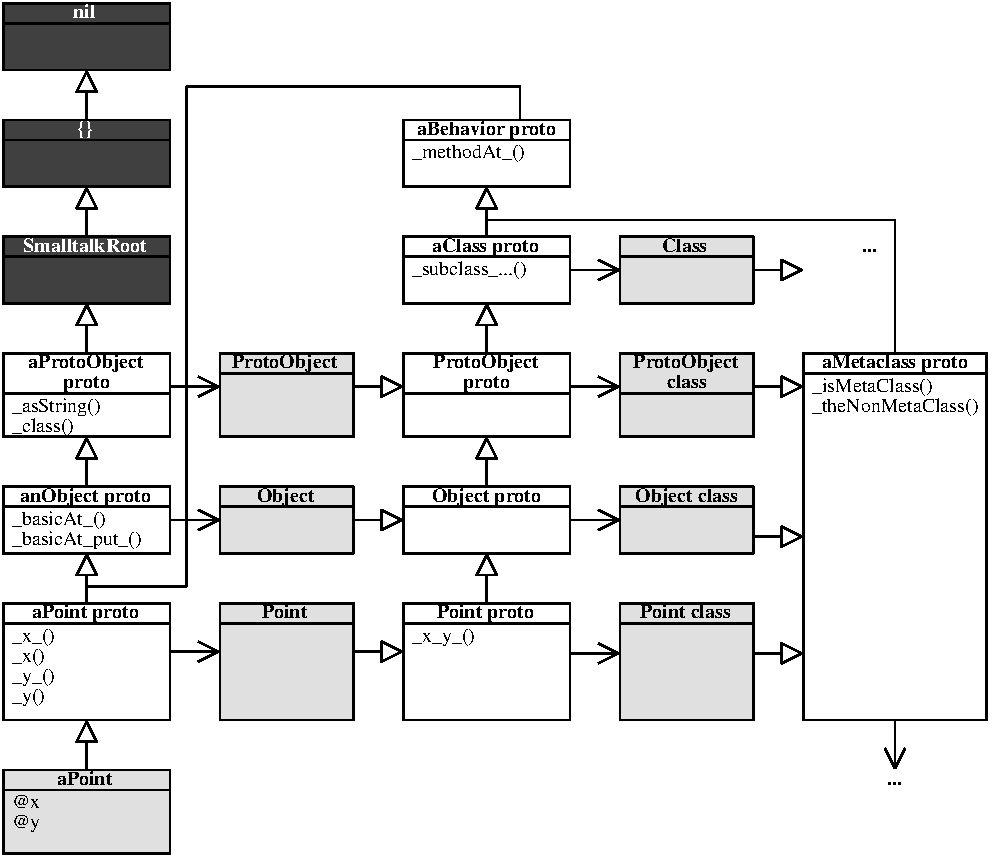
\includegraphics[width=0.45\textwidth]{amber_class_model}
\label{fig:amber_obj}
\caption{Part of Amber's object model as seen from the JavaScript side. Inheritance arrows designate prototype chains. An association arrow between object \texttt{a} and object \texttt{b} means that \texttt{a.klass = b}.}
\end{figure}

Figure~\ref{fig:amber_obj} shows a part of Amber Smalltalk's object model. As an example, consider the object \texttt{aPoint} which is an instance of the Smalltalk class \texttt{Point} and represents a 2D point with an x and a y coordinate. The corresponding instance variables are stored in \texttt{aPoint} directly. Its instance methods are stored in \texttt{aPoint proto}. All point instances have this object as a prototype. If we follow the prototype chain, we will get all of  \texttt{Point}'s super classes, and eventually reach an empty JavaScript object and, finally, \texttt{nil}. An object's class reference is stored in the JavaScript property \texttt{klass}. \texttt{ProtoObject proto}'s prototype is \texttt{aClass proto}, which is why every Smalltalk class is also \texttt{anObject}. Note, that \texttt{ProtoObject proto} corresponds to \texttt{ProtoObject}'s class side in Smalltalk, whereas \texttt{aClass proto} corresponds to \texttt{Class}' instance side in Smalltalk.


\section{COMPILATION PROCESS}
Amber Smalltalk compiles Smalltalk to JavaScript when a method is saved or a statement is executed in the workspace. In either case, the method \texttt{Compiler>>compile:} is called with the Smalltalk source code as an argument, and returns the JavaScript source code. The following list gives an overview of the compilation process.

\begin{enumerate}
    \item Smalltalk source code parsing: the parser is generated from a \emph{parsing expression grammar} using the PEG.js parser generator. The parser outputs an abstract syntax tree (AST).
    \item Semantic analysis: examples are checking if an identifier is defined (i.e., if a variable/class/argument/JavaScript variable with that name exists), or checking for variable shadowing which is not allowed in Smalltalk.
    \item AST to Intermediate Representation (IR) conversion: this step involves inlining message sends for \texttt{ifTrue:}, \texttt{ifFalse:}, \texttt{ifTrue:ifFalse:}, and \texttt{ifNil:ifNotNil:}.
    \item JavaScript code generation: JavaScript code is generated while traversing the IR tree.
\end{enumerate}

\section{OUR IMPLEMENTATION}
In this section, we describe the main ideas of our implementation. We first present an unoptimized implementation and will then show how to speed up our implementation.

\subsection{DATA STRUCTURE}
In context-oriented programming, we modularize partial methods in layers. Every partial method belongs to exactly one base method in a specific class. In ContextAmber, a layer is an instance of a subclass of the class \texttt{Layer}. We consider several alternatives for associating partial methods with base classes.

\paragraph{Class Name Prefix}
We create a class for every layer. The names of partial methods are a combination of the base class name and the base method name. Consider, for example, that we want to define a layer \texttt{RotationLayer} for the base method \texttt{Point>>x:}. The name of the partial method would be \texttt{RotationLayer>>Point\$x:}. The dollar sign has no meaning in Amber Smalltalk but is also not allowed in identifiers. Implementing this approach requires changing the grammar, such that the dollar sign is allowed in method names, and adding a check to the semantic analyzer that ensures that method names with a single dollar sign are allowed only in methods defined in a layer.

\paragraph{Method Protocols}
Instead of prefixing partial method names, the partial method's protocol is the name of the base class; however, this restricts us in categorizing partial methods in a meaningful way.

\paragraph{Partial Classes}
A layer definition consists of multiple classes. For every base class for which a partial method exists, there is a separate class containing all partial methods for that base class. We call these classes partial classes. In addition, there is a central layer class maintaining all layer-specific state and aggregating all partial classes for that layer. We use partial classes in ContextAmber, but other implementations typically use class name prefixes (e.g., JCop and ContextJS).

\subsection{LAYER ACTIVATION}
ContextAmber supports activating layers by default (also referred to as \emph{global} layer activation), object-wise layer activation, and scoped layer activation.

\paragraph{Default Layer Activation State}
A layer's default activation state defines whether a layer is activated or deactivated by default. Initially, all layers are deactivated by default. Object-wise and scoped layer activation can override a layer's default activation state; otherwise, the default activation state determines whether a layer is active or not. 

Our implementation maintains a stack of layers that are activated by default. A layer is being activated by default by adding it to the stack. Similarly, it is being deactivated by default by removing it from the stack (if present). Activating an already active layer or deactivating an already deactivated layer has no effect. Note, that the order in which we change the default activation state for multiple layers affects their composition order.

\paragraph{Object-wise Layer Activation}
A layer can be activated or deactivated on a per-object basis. Object-wise layer activation overrides default layer activation. Consider, for example, that layer $L1$ is already activated by default. If we deactivate layer $L1$ for an object $o$, $L1$ will not be part of the current layer composition when sending a message to $o$.

Every object maintains a single stack of layer activation and layer deactivation statements (denoted by \texttt{+layer} and \texttt{-layer}, respectively). We also support resetting a layer (denoted by \texttt{*layer}) which removes layer (de)activation statements from the stack. Resetting a layer means reverting its activation state to its default activation state, while deactivating a layer means turning off a layer for an object; even if it was activated both by default and for the current object. For example, let $D = (L1, L2, L3)$ be the default active layer stack and $O = (+L1, +L2, -L1, *L2, +L4)$ be the sequence of layer activation changes for an arbitrary object. Changing layers according to $O$ results in a layer (de)activation stack of $O' = (-L1, +L4)$. The resulting layer composition for $D$ and $O'$ is $(L2, L3, L4)$.

\paragraph{Scoped layer activation}
A layer can be activated or deactivated within a certain scope (i.e., within a block). Scoped layer activation overrides object-wise layer activation. Similar to object-wise layer activation, a layer can be activated, deactivated, or reset. Since JavaScript is single-threaded, it is sufficient to maintain a single stack of layer activation and deactivation statements for the current scope. This stack is modified before the block is executed, and reset to its original state after the block was executed.

\paragraph{Interface}
The following table gives an overview of the ContextAmber API for activating and deactivating layers.
\begin{table}[h]
\centering
\begin{tabular}{cc}
\multirow{2}{*}{Default} & \texttt{Layer>>activate} \\
 & \texttt{Layer>>deactivate} \\
 \hline
\multirow{3}{*}{Object-wise} & \texttt{Object>>activateLayer:} \\
 & \texttt{Object>>deactivateLayer:} \\
 & \texttt{Object>>resetLayer:} \\
 \hline
\multirow{3}{*}{Scoped} & \texttt{BlockClosure>>withLayer:} \\
 & \texttt{BlockClosure>>withoutLayer:} \\
 & \texttt{BlockClosure>>withResetLayer:} \\
\end{tabular}
\end{table}

\paragraph{Example}
The following table shows an example for calculating the layer composition when layers are activated by default, object-wise, and in the current scope.
\begin{table}[h]
\centering
\begin{tabular}{cccccc}
\multicolumn{2}{c}{default} & \multicolumn{2}{c}{object-wise} & \multicolumn{2}{c}{scoped} \\
instr. & stack & instr. & stack & instr. & stack \\
\hline
\texttt{+L1} & \texttt{+L4} & \texttt{+L1} & \texttt{-L2} & \texttt{-L1} & \texttt{+L2} \\
\texttt{+L2} & \texttt{+L2} & \texttt{+L3} & \texttt{+L1} & \texttt{-L1} & \texttt{-L2} \\
\texttt{-L1} &              & \texttt{+L2} &              & \texttt{*L1} & \texttt{-L4} \\
\texttt{-L3} &              & \texttt{*L3} &              & \texttt{-L4} & \\
\texttt{+L4} &              & \texttt{-L2} &              & \texttt{-L2} & \\
             &              &              &              & \texttt{+L2} & \\
\end{tabular}
\begin{tabular}{cc}
composed stack & \texttt{(+L2, +L4, +L1, -L2, -L4, -L2, +L2)} \\
layer composition & \texttt{(L1, L2)} \\
\end{tabular}
\end{table}

\subsection{LAYER/PARTIAL CLASS CREATION}
Layers and partial classes are classes defined through ContextAmber's API instead of the Smalltalk subclassing API. Partial classes are subclasses of \texttt{PartialClass} and contain a method \texttt{PartialClass class>>base} defining the base class. Layers are subclasses of \texttt{Layer} and contain a method \texttt{Layer class>>partialClasses} defining a collection of all partial classes. \texttt{Layer} instances have an ID which is unique among all layer instances of all layer classes. The layer ID is an inexpensive way of referencing layers, since Amber Smalltalk does not have the concept of an object ID. We use it to calculate the \emph{composition signature}, an integer value representing the current layer composition. The following listing shows the interface for defining layers and partial classes.

\begin{table}[h]
    \begin{tabular}{ll}
        \texttt{ContextAmber} & \texttt{newPartialClass: \#PartialClassName} \\
         & \texttt{baseClass: DemoClass} \\
         & \texttt{package: 'ContextAmber-Tests'} \\
       \\
        \texttt{ContextAmber} & \texttt{newLayer: \#LayerName} \\
        & \texttt{layerClasses: \{PartialClassName\}} \\
        & \texttt{instanceVariableNames: ''} \\
        & \texttt{package: 'ContextAmber-Tests'} 
    \end{tabular}
\end{table}

\subsection{IMPLEMENTATION DETAILS}
(this is a stub)

\paragraph{Wrapper Code Generation}
For a partial method, ContextAmber generates a wrapper (decorator) method replacing the corresponding base method, whenever the partial method is created for the first time or the base method changes. In the latter case, the new base method overwrites the wrapper method; therefore, we have to reinstall the wrapper method.

The wrapper method retrieves the current layer composition and invokes the corresponding partial method of the layer on top of the stack. The layer at the bottom of the stack is always the base class.

\paragraph{System Startup}
Amber Smalltalk is different from most Smalltalk implementations in a sense that the system state (image) cannot be saved and reloaded later. Amber Smalltalk bootstraps a minimal Smalltalk system and then loads all other classes. Only committed code (behavior) survives a reload, but not objects. Therefore, partial class to base class relationships and the per-layer collection of partial classes must be stored in methods instead of instance variables. Furthermore, ContextAmber has to reinstall all wrapper methods on startup.

\section{OPTIMIZATIONS}
In this section, we present optimizations which speed up ContextAmber.

\subsection{ASSUMPTIONS}
Most of the optimizations presented in this section are based on the assumption that method invocations are much more frequent than the layer composition changes~\cite{10.1109/C5.2012.20}. Therefore, we try to speed up the execution of layered methods at the cost of reduced performance for layer composition changes.

\subsection{INLINING PROCEED CALLS}
Layer compositions with a high number of layers and \texttt{proceed} calls slow down method execution, because every \texttt{proceed} call is an additional message send and requires finding the next layer from the stack of active layers. We speed up this process by replacing message sends of \texttt{proceed} selectors with the list of instructions of the corresponding partial method for the next layer in the IR tree.

\begin{figure}[!htp]
    \centering
    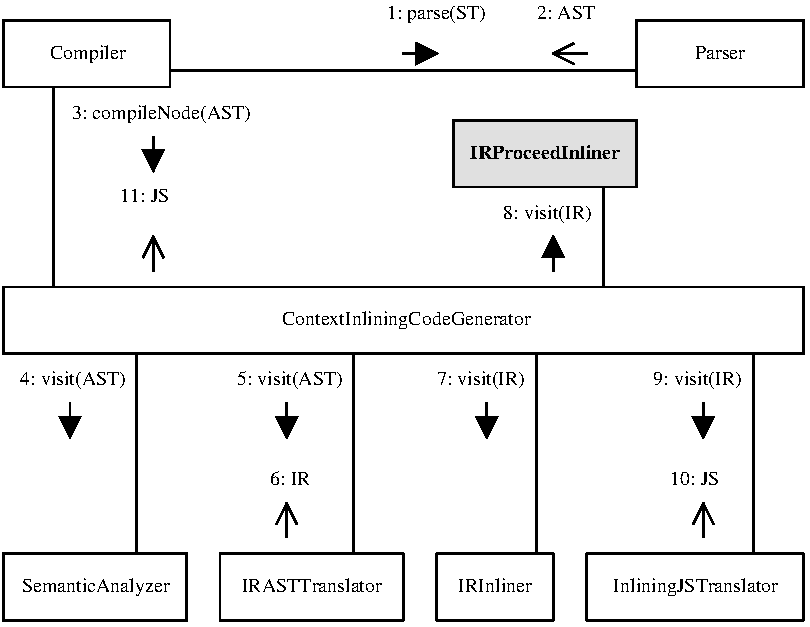
\includegraphics[width=0.45\textwidth]{compiler_inline.pdf}
    \label{fig:comp-inline}
    \caption{ContextAmber's integration into Amber Smalltalk's compiler infrastructure}
\end{figure}

ContextAmber adds another IR visitor to Amber's existing compiler infrastructure. The \texttt{IRProceedInliner} class inlines all \texttt{proceed} message sends. If an inlined partial method contains another \texttt{proceed} call, we will inline that one as well. The algorithm for this optimization is simple: we generate the IR for the base method, for the lowest layer, for the next higher layer, and so on, until we reach the layer on top of the stack. Every time we encounter a \texttt{proceed} call, we can immediately replace the send node with the instruction node containing the next partial method. By induction, that instruction node has already all \texttt{proceed} calls inlined.

\subsection{CACHING PARTIAL METHOD IR}
Whenever \texttt{IRProceedInliner} inlines partial methods, it parses the Smalltalk code and generates an AST and IR for all layers in the current layer composition. However, in many cases only the upper part of the layer composition stack changes. Therefore, it is sufficient to recompile partial methods beginning with the layer that changed.

In addition, we cache unoptimized IRs (i.e., without \texttt{proceed} inlining), such that we only have to parse Smalltalk code and generate AST and IR if the Smalltalk code changes. ContextAmber hooks into the Smalltalk compiler and stores the unoptimized IR in a JavaScript instance variable of the corresponding class object\footnote{This behavior is encapsulated in a layer, utilizing our framework.}. We store the IR tree in two cases.

\begin{itemize}
    \item The method is a partial method (i.e., it is part of a partial class).
    \item A partial method exists for the method being compiled (i.e., a partial class exists for the method's class, and that class has an implementation for the method's selector).
\end{itemize}

For the second case, ContextAmber has to go through all partial classes for a given class. Therefore, we store references to all partial classes in every base class. This collection of partial classes is updated when a partial class is added (subclassing \texttt{PartialClass}) and when a partial class is removed (utilizing a \texttt{SystemAnnouncer} callback).

\subsection{OBJECT-WISE METHOD INLINING}
When we inline proceed calls, we try to speed up the execution of layered methods by making the assumption that the layer composition is stable throughout a number of method invocations. At some point, the layer composition might change and inlined methods become invalid. We have to analyze the new layer composition and create a new inlined method. This is easy for global and scoped layers, because we can simply replace an instance method by its inlined version. For object-wise layer activation, we can have different layer compositions for objects of the same class and, therefore, different inlined methods. In the following paragraphs, we discuss several ideas for object-wise proceed inlining.

As a running example, consider that we have two objects \texttt{p1} and \texttt{p2}, both instances of \texttt{Point}. For \texttt{p1}, we activate \texttt{MetricLayer} which replaces the methods \texttt{x()} and \texttt{y()}, returning coordinates in the metric system. For \texttt{p2}, we activate \texttt{ImperialLayer} which replaces the same methods, returning coordinates in the imperial system. For every idea, we consider running \texttt{p1.x()}, \texttt{p2.x()}, \texttt{p1.x()} in that sequence.

\paragraph{Class-wide Method Inlining}
Inlined methods replace instance methods on the class level. When we run \texttt{p1.x()} for the first time, we replace \texttt{Point>>x} by an inlined method for \texttt{MetricLayer}. When we run \texttt{p2.x()}, we replace \texttt{Point>>x} by an inlined method for \texttt{ImperialLayer} because the layer composition is different now. Running \texttt{p1.x()} again replaces the method with the previous inlined method again.

\paragraph{Object-wide Method Inlining}
Inlined methods are stored on the object level. When we run \texttt{p1.x()} for the first time, we store the inlined method as \texttt{p1['\_x']} directly\footnote{Written in JavaScript notation since there is no Smalltalk notation for this.}. Respectively, we store inlined methods for \texttt{p2} as properties on \texttt{p2} directly. Running \texttt{p1.x()} again does not replace any methods, because the layer composition for \texttt{p1} did not change.

\paragraph{Class-wide Wrappers with Method Dictionaries}
A dictionary stores inlined methods, with one dictionary per base method. Every layered method is replaced by a wrapper method which calls retrieves the inlined method from the dictionary with the layer composition as the key, or creates and stores the inlined method in the dictionary if it does not exist. Let \texttt{l1} be the layer composition for \texttt{p1}, \texttt{l2} be the layer composition for \texttt{p2}, and \texttt{dictx} be the method dictionary for \texttt{Point>>x}. When we run \texttt{p1.x()} for the first time, we store the inlined method as \texttt{dictx[l1]} and call it. When we call the method on \texttt{p2}, we store it as \texttt{dictx[l2]}, respectively. Calling \texttt{p1.x()} again simply retrieves the method from \texttt{dictx} and calls it.

\paragraph{Cached Class-wide Method Inlining}
This is a combination of class-wide method inlining and method dictionaries, where inlined methods are cached in a method dictionary instead of reinlining them every time a method is replaced.

\paragraph{Cached Object-wide Method Inlining}
This is a combination of object-wide method inlining and method dictionaries, where inlined methods are cached in a method dictionary instead of reinlining them every time a method is replaced.

\paragraph{Hybrid Approach}
This variant combines multiple approaches and switches between them heuristically. For example, an implementation could use object-wide method inlining and switch to class-wide method inlining for a sepecific class at runtime, if a lot of instances of that class are created.

\subsection{INVALIDATING INLINED METHODS}
If the layer composition changes, we might have to throw away inlined methods and generate new ones. In this subsection, we discuss at what time a method could be reinlined.

\paragraph{On Layer Composition Change}
Every time we activate or deactivate a layer, we reinline all inlined methods for all partial methods associated with the layer (i.e., layer $\rightarrow$ partial classes $\rightarrow$ partial methods). Initially, all base methods for which partial methods exist, are replaced with dummy methods which replace itself with their inlined version on their first invocation. This ensures that we do not reinline inlined methods for methods which exist but are never invoked. 

Note, that for object-wide method inlining, a partial class has to know all of its base class' instances (recall that inlined methods are stored in the object itself), which could be a large number and cause memory leaks. 

\paragraph{On Method Invocation}
Every inlined method stores the layer composition for which it was created and checks if its layer composition is the same as the current layer composition for the object when it is invoked. Note, that every time we call an inlined method, we have to recalculate the stack of active layers for the object.

\paragraph{On Method Invocation with Dirty Flag}
Every inlined method stores a dirty flag indicating if the inlined method is up to date with respect to the current layer composition. The dirty flag is set whenever the layer composition changes in the same way as we reinline methods on layer composition change. Note, that for object-wide method inlining, a partial class has to know all of its base class' instances, in order to set the dirty bit on their methods.

\paragraph{On Method Invocation with Dirty Flag and Versions}
This is an optimization of the previous approach which does not require partial classes to have references to all of its base class' instances for object-wide method inlining. Every inlined method stores a dirty flag indicating if it is up to date with respect to the object's layer composition (i.e., the dirty flag is set whenever a layer is activated or deactivated for the object the method belongs to). Whenever the global or scoped layer composition stack changes, all dirty bits remain unchanged. In addition to the dirty bit, every inlined method stores a single version number for the global and scoped layer composition stack. Every time the global or scoped layer composition stack changes, a global version number is incremented. Inlined methods check the dirty bit and compare their version number. If either one of them indicates that the method is out of date, it is reinlined.

\paragraph{Example}
Figure~\ref{fig:inlining-example} illustrates ContextAmber's data structure for invalidating inlined methods. ContextAmber supports cached class-wide and object-wide method inlining, and invalidates inlined methods on method invocation with dirty flag and optionally with a version number. Method execution statistics and heuristics decide when ContextAmber switches between these variants.

\begin{figure}[!htp]
    \centering
    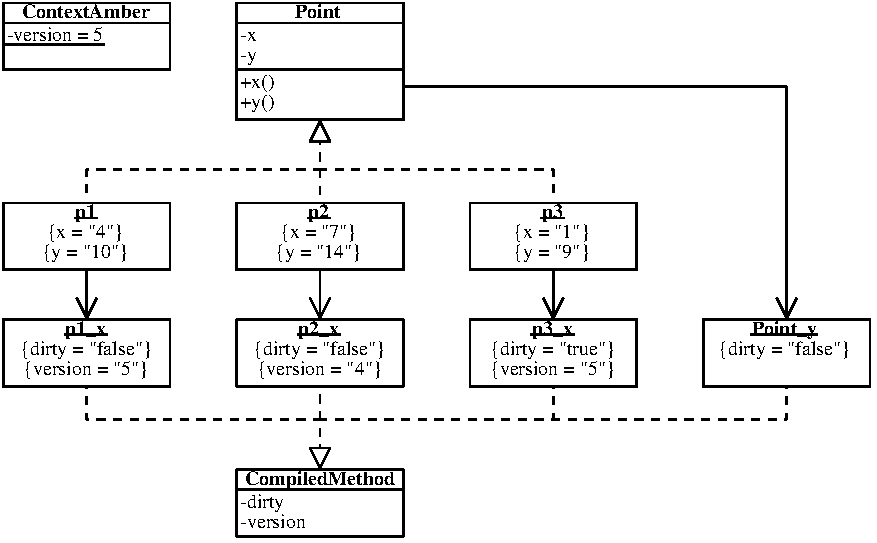
\includegraphics[width=0.45\textwidth]{inlining_example.pdf}
    \label{fig:inlining-example}
    \caption{ContextAmber's data structure for invalidating inlined methods}
\end{figure}

In our example, \texttt{Point>>x} is inlined object-wide, whereas \texttt{Point>>y} is inlined class-wide, since in this example we assume that the behavior of the former method changes quite often due to object-wide layer composition changes, whereas the latter method changes infrequently. Calling \texttt{p2.x()} causes reinlining \texttt{p2}'s method because its version number is outdated (i.e., a global or scoped layer affecting \texttt{Point>>x} was activated or deactivated). Calling \texttt{p3.x()} causes reinlining \texttt{p3}'s method because it is marked dirty (i.e., a layer affecting \texttt{p3.x} was activated or deactivated). Calling \texttt{p1.x()} or any \texttt{y()} method does not cause any reinlining because these methods are not outdated.
\section{PROFILING SMALLTALK METHODS}
Talk about the Smalltalk method profiler.

\section{FUTURE WORK}
Talk about what still needs to be done.

\section{CONCLUSION}

\bibliography{contextamber}{}
\bibliographystyle{plain}

\end{document}
